% Provenance (never printed): see sources/outline_sources.md (Year 1: the wind-driven
% circulation, gyres, Ekman transport and upwelling, western boundary currents, the
% meridional overturning circulation and the water masses). Exercise and problem values in
% the Book 3 scratch calculator calc/ch29.py; figures from figdata/bachelor-1/
% ekman_hodograph.py (Ekman's solution with Ekman's constants) and stommel_gyre.py
% (Stommel's 1948 model, exercise parameters), the world map from figdata/shared/geo.py.
% Physics owns the Coriolis force (recalled). Book 1 (g8) gave the surface currents and
% the gyres in words, Book 2 (g10) upwelling: re-founded here with the Ekman balance.
% Ch. 26 owns the T-S diagram and the water masses, ch. 28 the Coriolis parameter, the
% geostrophic wind and the mean meridional streamfunction. The Sverdrup balance, the
% vorticity argument and the derivation of the Ekman spiral are the Year 3 volume's; ENSO
% the Year 2 volume's.
\chapter{La circulación del océano}\label{ch:b1:ocean-circulation}

En 1992, durante una tormenta en el Pacífico Norte, un contenedor cayó por la borda de un barco que navegaba de Hong Kong a Estados Unidos. Se abrió y liberó unos \num{29000} patos de goma y otros juguetes de baño, que flotaron lejos y viajaron muy lejos; los lugares donde algunos de ellos aparecieron después ayudaron a los científicos a entender las corrientes que los habían llevado. Los juguetes flotantes siguen el agua de la superficie, y el agua superficial de los océanos no vaga al azar: gira en \omterm{def:b1:ocean-circulation:gyre}{giros} de toda la cuenca, corre hacia el norte en corrientes estrechas a lo largo de las costas occidentales de los océanos, y asciende o desciende en unos pocos lugares elegidos. Este capítulo explica cómo el viento pone en movimiento la capa superior del océano, por qué el agua se mueve en ángulo recto con el viento que la empuja, por qué las corrientes más fuertes se pegan a los lados occidentales de los océanos, y cómo un vuelco lento lleva agua hasta el abismo y de vuelta.
% ledger: noaa:floatees

\begin{omfigure}
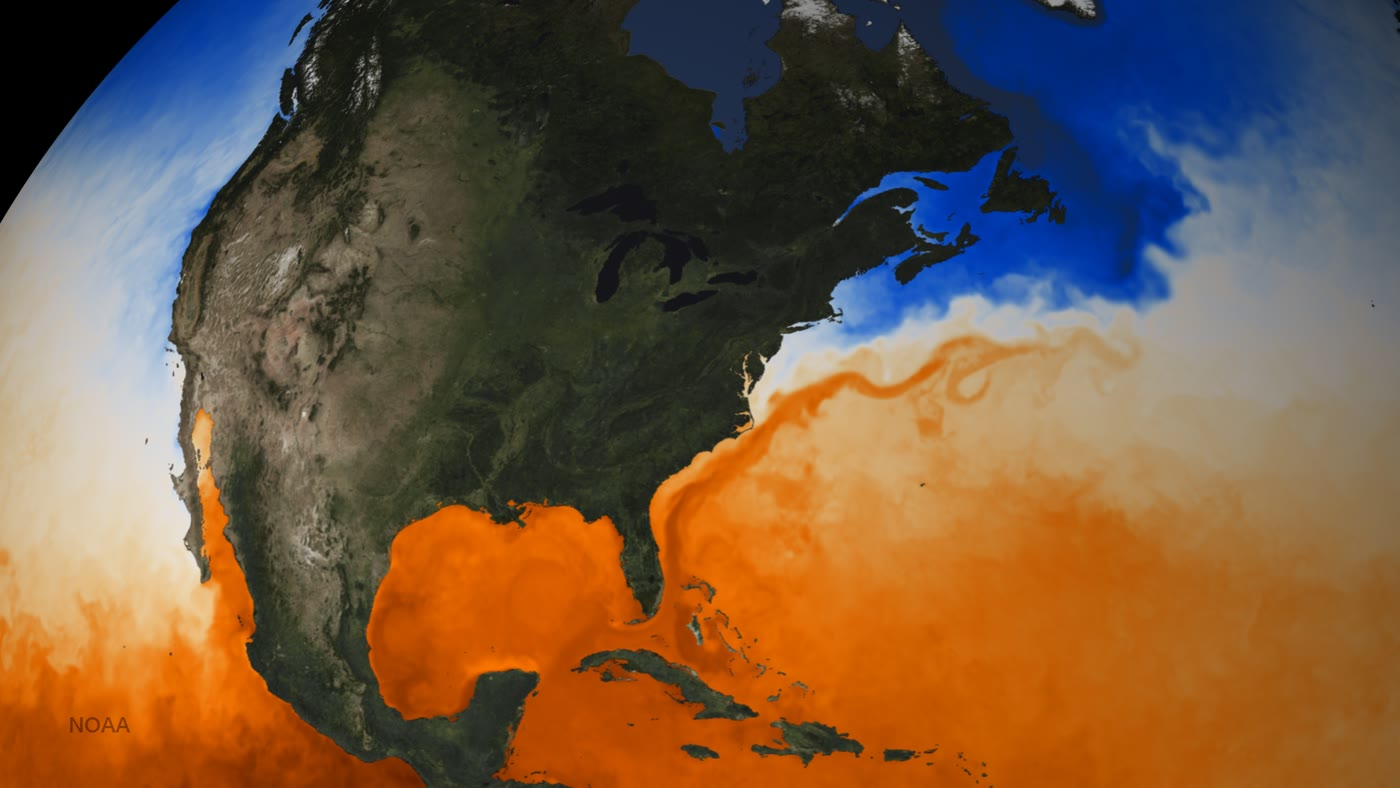
\includegraphics[width=0.85\linewidth]{images/book3/b1-gulf-stream-sst.jpg}

{\small La temperatura de la superficie del mar alrededor de Norteamérica a principios de junio de 2016, a partir de datos de satélite (agua cálida en naranja, agua fría en azul). La corriente del Golfo sale de la costa de Estados Unidos como una cinta cálida y serpenteante y cruza el Atlántico hacia Europa; a las mismas \omterm{def:b1:spherical-astronomy:geographic}{latitudes}, el agua frente a la costa del Pacífico es mucho más fría que frente a la del Atlántico. (NOAA, NESDIS, dominio público, vía Wikimedia Commons.)}
\label{fig:b1:ocean-circulation:sst}
\end{omfigure}
% ledger: commons:gulf-stream-sst, noaa:gulf-stream-heat

\begin{recall}
Los libros de física dan la fuerza de Coriolis. \Cref{ch:b1:atmospheric-circulation}
escribió su parte horizontal como $-f\,\vec k\times\vec v$, con el \omterm{def:b1:atmospheric-circulation:coriolis-parameter}{parámetro de Coriolis}
$f = 2\Omega\sin\varphi$ ($\Omega = \qty{7.292e-5}{rad.s^{-1}}$), y halló los \omterm{def:b1:atmospheric-circulation:winds}{alisios}, los levantes entre el ecuador y unos \ang{30}, y los \omterm{def:b1:atmospheric-circulation:winds}{vientos del oeste} más allá; también definió la \omterm{def:b1:atmospheric-circulation:streamfunction}{función de corriente meridional media} de un vuelco.
\Cref{ch:b1:fluid-envelopes-structure} dio la \omterm{def:b1:fluid-envelopes-structure:ocean-layers}{capa de mezcla} y la \omterm{def:b1:fluid-envelopes-structure:ocean-layers}{termoclina}, la densidad del agua de mar, el \omterm{def:b1:fluid-envelopes-structure:ts-diagram}{diagrama T--S} y las \omterm{def:b1:fluid-envelopes-structure:ts-diagram}{masas de agua} del Atlántico Sur, y \cref{ch:b1:radiation-heat-transport} el transporte de calor hacia los polos que comparten la atmósfera y el océano. El libro 1 describió las corrientes superficiales y los grandes \omterm{def:b1:ocean-circulation:gyre}{giros}; el libro 2, el \omterm{def:b1:ocean-circulation:upwelling}{afloramiento} de agua fría a lo largo de algunas costas.
% ledger: earth:Trot, nos:gyres
\end{recall}

\section{El viento y las corrientes superficiales}\label{sec:b1:ocean-circulation:wind}

El viento mueve el mar por fricción. Su fuerza se reparte sobre la superficie, y se mide, como una presión, por unidad de área.

\begin{definition}[Tensión del viento]\label{def:b1:ocean-circulation:wind-stress}
La \emph{tensión del viento}\index{tensión del viento} $\vec T$ es la fuerza horizontal por unidad de área que ejerce el viento sobre la superficie del mar, en pascales. Es la transferencia hacia abajo del momento horizontal del aire hacia el océano, y apunta casi a lo largo del viento. Su tamaño viene dado por la fórmula de masa,
\[
  T = \rho_a C_D U_{10}^2,
\]
donde $\rho_a = \qty{1.3}{kg.m^{-3}}$ es la densidad del aire, $U_{10}$ la rapidez del viento a \qty{10}{m} sobre el mar y $C_D$ un coeficiente de arrastre adimensional.
\end{definition}
% ledger: stewart:wind-stress

El coeficiente de arrastre se mide con instrumentos rápidos que registran las fluctuaciones turbulentas del viento a unos metros sobre las olas. Para un aire de estabilidad neutra, las medidas de Yelland y Taylor dan
\[
  1000\,C_D = 0.29 + \frac{3.1}{U_{10}} + \frac{7.7}{U_{10}^2}
  \quad (\qtyrange{3}{6}{m/s}),
  \qquad
  1000\,C_D = 0.60 + 0.071\,U_{10}
  \quad (\qtyrange{6}{26}{m/s}),
\]
con $U_{10}$ en metros por segundo. Un viento de \qty{10}{m/s} tiene $C_D =
\num{1.31e-3}$ y ejerce $T = 1.3 \times \num{1.31e-3} \times 100 =
\qty{0.170}{Pa}$; un viento de \qty{5}{m/s}, \qty{0.040}{Pa}; un temporal de
\qty{20}{m/s}, \qty{1.05}{Pa}. Duplicar el viento de 10 a \qty{20}{m/s} multiplica la tensión por $6.2$, no por $4$: los mares más rugosos agarran el viento con más fuerza. Estas tensiones son minúsculas, una millonésima de la presión atmosférica, pero actúan sin pausa sobre todo el océano.
% ledger: stewart:drag-coefficient (computed in figdata/bachelor-1/ekman_hodograph.py and calc/ch29.py)

El patrón de la tensión sigue al de los vientos. Entre los \omterm{def:b1:atmospheric-circulation:winds}{alisios} de los trópicos, que soplan hacia el oeste, y los \omterm{def:b1:atmospheric-circulation:winds}{vientos del oeste} de las \omterm{def:b1:spherical-astronomy:geographic}{latitudes} medias, que soplan hacia el este, el agua superficial de cada cuenca oceánica se pone a girar.

\begin{definition}[Giro; giros subtropicales y subpolares]\label{def:b1:ocean-circulation:gyre}
Un \emph{giro}\index{giro} es un gran sistema de corrientes oceánicas en rotación que llena una cuenca oceánica. Un \emph{giro subtropical}\index{giro subtropical} yace entre los \omterm{def:b1:atmospheric-circulation:winds}{alisios} y los \omterm{def:b1:atmospheric-circulation:winds}{vientos del oeste}, y gira en sentido horario en el hemisferio norte y en sentido antihorario en el sur. Un \emph{giro subpolar}\index{giro subpolar} yace en el lado hacia el polo de los \omterm{def:b1:atmospheric-circulation:winds}{vientos del oeste} y gira en sentido contrario.
\end{definition}
% ledger: nos:gyre-def, nos:boundary-currents, stewart:north-atlantic

Hay cinco \omterm{def:b1:ocean-circulation:gyre}{giros subtropicales}, en el Atlántico Norte y Sur, el Pacífico Norte y Sur y el océano Índico; ninguno cruza el ecuador. En el Atlántico Norte, el \omterm{def:b1:ocean-circulation:gyre}{giro subtropical} queda cerrado por la corriente del Golfo a lo largo de la costa de Estados Unidos, en el oeste, y por la corriente de Canarias frente a África, en el este; al norte de él, el \omterm{def:b1:ocean-circulation:gyre}{giro subpolar} gira en sentido antihorario, con la corriente del Atlántico Norte en su lado sur y la corriente de Labrador que fluye hacia el sur por su lado oeste. A bajas \omterm{def:b1:spherical-astronomy:geographic}{latitudes}, las corrientes ecuatoriales hacia el oeste del Atlántico y del Pacífico están separadas por una contracorriente hacia el este. Los \omterm{def:b1:ocean-circulation:gyre}{giros} no son simétricos: cada \omterm{def:b1:ocean-circulation:gyre}{giro subtropical} está cerrado por una corriente fuerte y estrecha en el lado occidental de su cuenca y por una corriente débil y ancha en el lado oriental. Alrededor de la Antártida, donde ningún continente lo detiene, la corriente circumpolar antártica fluye hacia el este alrededor del globo, impulsada por los \omterm{def:b1:atmospheric-circulation:winds}{vientos del oeste} del océano Austral.
% ledger: nos:boundary-currents, stewart:north-atlantic, stewart:heat-conveyor, lien:kuroshio, donohue:acc, stewart:acc

\begin{omfigure}
\begin{tikzpicture}
\begin{axis}[ommap, width=0.98\linewidth, xtick={-180,-120,...,180}, ytick={-60,-30,0,30,60}]
% land: figdata/shared/geo.py; ledger: data:ne-land. Arrows placed by hand from the
% ledgered pattern: nos:boundary-currents, stewart:north-atlantic, lien:kuroshio,
% donohue:acc, stewart:acc
\addplot[fill=omLithAlluv, draw=black!45, line width=0.2pt, forget plot] table {figdata/out/shared-geo-land.dat};
% North Atlantic subtropical gyre (clockwise)
\addplot[omThm, line width=1.1pt, -{Stealth[length=4pt]}, smooth] coordinates {(-80,26) (-77,32) (-70,37) (-58,40) (-44,41)};
\addplot[omThm, line width=1.1pt, -{Stealth[length=4pt]}, smooth] coordinates {(-38,40) (-28,39) (-20,36)};
\addplot[omThm, line width=1.1pt, -{Stealth[length=4pt]}, smooth] coordinates {(-19,32) (-21,24) (-26,17)};
\addplot[omThm, line width=1.1pt, -{Stealth[length=4pt]}, smooth] coordinates {(-32,14) (-45,13) (-60,15)};
% North Atlantic subpolar gyre (anticlockwise)
\addplot[omDef, line width=1.1pt, -{Stealth[length=4pt]}, smooth] coordinates {(-40,47) (-28,52) (-18,57)};
\addplot[omDef, line width=1.1pt, -{Stealth[length=4pt]}, smooth] coordinates {(-24,61) (-35,62) (-44,59)};
\addplot[omDef, line width=1.1pt, -{Stealth[length=4pt]}, smooth] coordinates {(-55,59) (-56,53) (-51,47)};
% North Pacific subtropical gyre (clockwise)
\addplot[omThm, line width=1.1pt, -{Stealth[length=4pt]}, smooth] coordinates {(123,19) (125,26) (133,32) (143,36) (156,38)};
\addplot[omThm, line width=1.1pt, smooth] coordinates {(162,39) (172,40) (180,40.5)};
\addplot[omThm, line width=1.1pt, -{Stealth[length=4pt]}, smooth] coordinates {(-180,40.5) (-165,41) (-148,40)};
\addplot[omThm, line width=1.1pt, -{Stealth[length=4pt]}, smooth] coordinates {(-133,37) (-128,29) (-122,20)};
\addplot[omThm, line width=1.1pt, -{Stealth[length=4pt]}, smooth] coordinates {(-125,13) (-150,12) (-175,13)};
\addplot[omThm, line width=1.1pt, -{Stealth[length=4pt]}, smooth] coordinates {(170,13) (152,14) (135,15)};
% South Atlantic subtropical gyre (anticlockwise)
\addplot[omThm, line width=1.1pt, -{Stealth[length=4pt]}, smooth] coordinates {(2,-8) (-15,-9) (-30,-9)};
\addplot[omThm, line width=1.1pt, -{Stealth[length=4pt]}, smooth] coordinates {(-34,-14) (-39,-24) (-47,-34)};
\addplot[omThm, line width=1.1pt, -{Stealth[length=4pt]}, smooth] coordinates {(-42,-40) (-20,-40) (2,-38)};
\addplot[omThm, line width=1.1pt, -{Stealth[length=4pt]}, smooth] coordinates {(10,-31) (9,-23) (6,-15)};
% South Pacific subtropical gyre (anticlockwise)
\addplot[omThm, line width=1.1pt, -{Stealth[length=4pt]}, smooth] coordinates {(-88,-10) (-120,-11) (-160,-12)};
\addplot[omThm, line width=1.1pt, -{Stealth[length=4pt]}, smooth] coordinates {(160,-16) (157,-26) (162,-35)};
\addplot[omThm, line width=1.1pt, -{Stealth[length=4pt]}, smooth] coordinates {(-170,-40) (-140,-41) (-105,-39)};
\addplot[omThm, line width=1.1pt, -{Stealth[length=4pt]}, smooth] coordinates {(-82,-36) (-82,-27) (-85,-17)};
% Indian Ocean subtropical gyre (anticlockwise)
\addplot[omThm, line width=1.1pt, -{Stealth[length=4pt]}, smooth] coordinates {(98,-13) (80,-14) (60,-15)};
\addplot[omThm, line width=1.1pt, -{Stealth[length=4pt]}, smooth] coordinates {(47,-22) (40,-29) (33,-34)};
\addplot[omThm, line width=1.1pt, -{Stealth[length=4pt]}, smooth] coordinates {(50,-38) (75,-37) (100,-35)};
\addplot[omThm, line width=1.1pt, -{Stealth[length=4pt]}, smooth] coordinates {(108,-31) (106,-24) (102,-18)};
% Antarctic Circumpolar Current (eastward)
\addplot[omMeth, line width=1.4pt, -{Stealth[length=5pt]}, smooth] coordinates {(-62,-58) (-40,-55) (-15,-52)};
\addplot[omMeth, line width=1.4pt, -{Stealth[length=5pt]}, smooth] coordinates {(5,-52) (40,-50) (75,-50)};
\addplot[omMeth, line width=1.4pt, -{Stealth[length=5pt]}, smooth] coordinates {(95,-51) (130,-53) (165,-56)};
\addplot[omMeth, line width=1.4pt, -{Stealth[length=5pt]}, smooth] coordinates {(-170,-58) (-130,-59) (-85,-59)};
\node[font=\scriptsize, anchor=west, fill=white, fill opacity=0.8, text opacity=1, inner sep=1pt] at (axis cs:-66,31) {corriente del Golfo};
\node[font=\scriptsize, anchor=west, fill=white, fill opacity=0.8, text opacity=1, inner sep=1pt] at (axis cs:-11,25) {Canarias};
\node[font=\scriptsize, anchor=east, fill=white, fill opacity=0.8, text opacity=1, inner sep=1pt] at (axis cs:-58,52) {Labrador};
\node[font=\scriptsize, anchor=west, fill=white, fill opacity=0.8, text opacity=1, inner sep=1pt] at (axis cs:142,28) {Kuroshio};
\node[font=\scriptsize, anchor=north, fill=white, fill opacity=0.8, text opacity=1, inner sep=1pt] at (axis cs:-150,9) {Ecuatorial Norte};
\node[font=\scriptsize, anchor=north, fill=white, fill opacity=0.8, text opacity=1, inner sep=1pt] at (axis cs:0,-62) {Corriente Circumpolar Antártica};
\end{axis}
\end{tikzpicture}

{\small Los \omterm{def:b1:ocean-circulation:gyre}{giros} del océano superficial (flechas esquemáticas sobre un mapa de tierras). Rojo oscuro: los cinco \omterm{def:b1:ocean-circulation:gyre}{giros subtropicales}, en sentido horario en el hemisferio norte y antihorario en el sur, cada uno con una corriente estrecha de frontera occidental; azul: el \omterm{def:b1:ocean-circulation:gyre}{giro subpolar} del Atlántico Norte; verde: la corriente circumpolar antártica. Solo se nombran las corrientes tratadas en el texto. Las flechas muestran el sentido del flujo, no su rapidez.}
\label{fig:b1:ocean-circulation:gyres}
\end{omfigure}
% ledger: data:ne-land, nos:boundary-currents, stewart:north-atlantic, lien:kuroshio, donohue:acc

Dos rasgos de este patrón necesitan explicación. El primero es el sentido de \omterm{def:b1:ocean-circulation:gyre}{giro}: los \omterm{def:b1:atmospheric-circulation:winds}{alisios} soplan hacia el oeste en el lado del ecuador de un \omterm{def:b1:ocean-circulation:gyre}{giro subtropical}, y sin embargo las corrientes del \omterm{def:b1:ocean-circulation:gyre}{giro} no siguen simplemente a los vientos, y el agua superficial deriva en ángulo respecto a ellos. El segundo es la asimetría: el flujo de retorno de un \omterm{def:b1:ocean-circulation:gyre}{giro} se comprime contra el lado occidental de su cuenca. Ambos vienen de la rotación de la Tierra.

\section{Transporte de Ekman}\label{sec:b1:ocean-circulation:ekman}

\begin{history}[Nansen y Ekman, 1898--1905]
Durante su expedición en el Ártico, Fridtjof Nansen observó que el viento empujaba el hielo marino no a lo largo del viento, sino con un ángulo de \ang{20} a \ang{40} a su derecha, mirando hacia donde sopla el viento. Razonó que tres fuerzas debían equilibrarse sobre el hielo en movimiento: el empuje del viento, la fricción del agua y la fuerza de Coriolis. Pidió al meteorólogo Vilhelm Bjerknes que dejara a uno de sus estudiantes estudiar la influencia de la rotación terrestre sobre las corrientes impulsadas por el viento. El estudiante, Walfrid Ekman, elaboró la teoría para su tesis doctoral en Uppsala, y la amplió en 1905. Su solución sigue siendo el punto de partida de la teoría del océano impulsado por el viento.
\end{history}
% ledger: stewart:ekman-layer, nos:ekman-spiral

\begin{definition}[Capa de Ekman, transporte de Ekman, espiral de Ekman]\label{def:b1:ocean-circulation:ekman}
La \emph{capa de Ekman}\index{capa de Ekman} es la capa superficial delgada del océano, como mucho de unos pocos cientos de metros de espesor, en la que la \omterm{def:b1:ocean-circulation:wind-stress}{tensión del viento} se transmite hacia abajo por fricción turbulenta y se equilibra con la fuerza de Coriolis. El \emph{transporte de
Ekman}\index{transporte de Ekman} es la \omterm{def:b1:fluid-envelopes-structure:ts-diagram}{masa de agua} que la capa lleva por segundo a través de una franja vertical de \qty{1}{m} de ancho, desde la superficie hasta por debajo de la capa:
\[
  \vec M = \int_{-d}^{0} \rho\,\vec v\,\mathrm dz \quad (\unit{kg.m^{-1}.s^{-1}});
\]
dividida por la densidad, es un transporte de volumen por metro, en
\unit{m^2.s^{-1}}. La \emph{espiral de Ekman}\index{espiral de Ekman} es el \omterm{def:b1:ocean-circulation:gyre}{giro} y debilitamiento de la corriente con la profundidad en la capa. Los transportes oceánicos se cuentan en \emph{sverdrups}\index{sverdrup (unidad)}: \qty{1}{\sverdrup} $=
\qty{e6}{m^3.s^{-1}}$.
\end{definition}
% ledger: stewart:ekman-layer, stewart:ekman-transport

\begin{theorem}[Transporte de Ekman]\label{thm:b1:ocean-circulation:ekman}
En estado estacionario, lejos de las costas, sobre agua mucho más profunda que la \omterm{def:b1:ocean-circulation:ekman}{capa de Ekman}, el \omterm{def:b1:ocean-circulation:ekman}{transporte de Ekman} depende solo de la \omterm{def:b1:ocean-circulation:wind-stress}{tensión del viento} $\vec T$ y del \omterm{def:b1:atmospheric-circulation:coriolis-parameter}{parámetro de Coriolis} $f$:
\[
  \vec M = \frac{1}{f}\,\vec T\times\vec k,
  \qquad |\vec M| = \frac{|\vec T|}{|f|}.
\]
Es perpendicular a la \omterm{def:b1:ocean-circulation:wind-stress}{tensión del viento}, a su derecha en el hemisferio norte y a su izquierda en el sur.
\end{theorem}
% ledger: stewart:ekman-transport

\begin{proof}
Sea $\vec\tau(z)$ la tensión horizontal que el agua por encima del nivel $z$ ejerce sobre el agua de debajo. En la superficie es la \omterm{def:b1:ocean-circulation:wind-stress}{tensión del viento}, $\vec\tau(0) =
\vec T$; por debajo de la capa, donde las corrientes impulsadas por el viento se han extinguido, se anula, $\vec\tau(-d) = \vec 0$. Una losa delgada entre $z$ y $z + \mathrm dz$, de área horizontal unitaria, recibe $\vec\tau(z + \mathrm dz)$ en su cara superior y
$-\vec\tau(z)$ en su cara inferior: la fuerza de fricción neta es $(\partial\vec
\tau/\partial z)\,\mathrm dz$. Su masa es $\rho\,\mathrm dz$, y la fuerza horizontal de Coriolis sobre ella es $-f\,\vec k\times\vec v\,\rho\,\mathrm dz$. En estado estacionario, sin cambio horizontal de un lugar a otro, las dos se equilibran:
\[
  -f\rho\,\vec k\times\vec v + \frac{\partial\vec\tau}{\partial z} = \vec 0 .
\]
Integrando de $-d$ a $0$,
\[
  -f\,\vec k\times\vec M + \vec\tau(0) - \vec\tau(-d) = \vec 0,
  \qquad\text{es decir}\qquad \vec k\times\vec M = \frac{\vec T}{f}.
\]
Para un vector horizontal, $\vec k\times(\vec k\times\vec M) = -\vec M$; tomando
$\vec k\times$ de ambos lados se obtiene $-\vec M = \vec k\times\vec T/f$, así que $\vec M =
\vec T\times\vec k/f$. El vector $\vec T\times\vec k$ es $\vec T$ girado
\ang{90} en sentido horario visto desde arriba: a la derecha del viento cuando $f > 0$, a la izquierda cuando $f < 0$. Su tamaño es $|\vec T|$.
\end{proof}

El resultado no depende de cómo funciona la fricción dentro de la capa, que se conoce mal: solo entran la tensión en el tope y su anulación en el fondo. Esto hace el transporte mucho más robusto que las velocidades mismas. El agua de toda la capa, tomada en conjunto, se mueve en ángulo recto con el viento, un resultado que parece extraño hasta recordar que, en un día o más, la fuerza de Coriolis tiene tiempo de girar cada corriente.

\begin{example}[El transporte bajo una brisa fresca]\label{ex:b1:ocean-circulation:transport}
Un viento de \qty{10}{m/s} que sopla hacia el norte a \ang{35} N ejerce $T = \qty{0.170}{Pa}$. Con $f = 2\Omega\sin\ang{35} = \qty{8.365e-5}{s^{-1}}$, el \omterm{def:b1:ocean-circulation:ekman}{transporte de Ekman} es $0.170/(\num{8.365e-5}) = \qty{2036}{kg.m^{-1}.s^{-1}}$, hacia el este. Con $\rho = \qty{1027}{kg.m^{-3}}$, son \qty{1.98}{m^3.s^{-1}} por cada metro medido a través del transporte: a través de una línea de \qty{1000}{km} de largo, unos \qty{2}{\sverdrup}.
\end{example}
% ledger: stewart:drag-coefficient, stewart:ekman-constants, earth:Trot (computed in calc/ch29.py)

La teoría se ha puesto a prueba en el mar. A \ang{11} N en el Atlántico, donde los \omterm{def:b1:atmospheric-circulation:winds}{alisios} soplan hacia el oeste, el \omterm{def:b1:ocean-circulation:ekman}{transporte de Ekman} es hacia el norte; medido directamente con un perfilador de corrientes, resultó ser \qty[uncertainty-mode=separate]{12.0 \pm 5.5}{\sverdrup}, frente a \qty[uncertainty-mode=separate]{8.8 \pm 1.9}{\sverdrup} calculado a partir de los vientos medidos durante la campaña y \qty[uncertainty-mode=separate]{13.5 \pm 0.3}{\sverdrup} a partir de vientos promediados a lo largo de muchos años.
% ledger: stewart:ekman-transport

Cómo se reparte la corriente con la profundidad dentro de la capa depende de la fricción. Ekman tomó el modelo más simple, una fricción turbulenta proporcional a la cizalla vertical de la corriente, $\vec\tau = \rho A_z\,\partial\vec v/\partial z$, con una viscosidad de remolino $A_z$ constante.

\begin{proposition}[La espiral de Ekman]\label{prop:b1:ocean-circulation:spiral}
Para una tensión de viento estacionaria $T$ hacia el norte sobre un océano profundo y homogéneo en el hemisferio norte, con una viscosidad de remolino $A_z$ constante, la corriente a la altura $z
\leq 0$ es
\[
  u = V_0\,e^{az}\cos\Bigl(\frac\pi4 + az\Bigr),\qquad
  v = V_0\,e^{az}\sin\Bigl(\frac\pi4 + az\Bigr),\qquad
  a = \sqrt{\frac{f}{2A_z}},\quad V_0 = \frac{T}{\rho\sqrt{fA_z}},
\]
con $u$ hacia el este y $v$ hacia el norte. En la superficie la corriente fluye a \ang{45} a la derecha del viento; con la profundidad se debilita como $e^{az}$ y gira aún más a la derecha. A la profundidad $D_E = \pi/a$, la profundidad de Ekman, fluye en contra de la corriente de superficie con $e^{-\pi} = \num{0.043}$ de su rapidez.
\end{proposition}
\admitted
% ledger: stewart:ekman-solution

La deducción resuelve las dos ecuaciones $f v + A_z u'' = 0$ y $-f u + A_z v'' =
0$ del equilibrio de la demostración anterior; se hace en el volumen de tercer año, y
\cref{exo:b1:ocean-circulation:10} comprueba que las fórmulas satisfacen las ecuaciones y que la espiral lleva exactamente el transporte del teorema. Para usar la espiral se necesita $A_z$, que no se mide directamente. Ekman reunió las velocidades observadas de las corrientes superficiales y encontró, para $|\varphi| \geq \ang{10}$,
\[
  V_0 = \frac{0.0127\,U_{10}}{\sqrt{\sin|\varphi|}},
  \qquad\text{que da}\qquad
  D_E = \frac{7.6\,U_{10}}{\sqrt{\sin|\varphi|}},
\]
en unidades del SI, con su coeficiente de arrastre $C_D = \num{2.6e-3}$ y $\rho_a =
\qty{1.25}{kg.m^{-3}}$. A \ang{35} N bajo un viento de \qty{10}{m/s}, $D_E =
\qty{100}{m}$ y $V_0 = \qty{0.17}{m/s}$; la \omterm{def:b1:ocean-circulation:ekman}{capa de Ekman} va desde unos
\qty{45}{m} con vientos suaves en \omterm{def:b1:spherical-astronomy:geographic}{latitudes} medias hasta \qty{300}{m} bajo un temporal en los trópicos, y la corriente de superficie es el \qtyrange{1}{2.5}{\percent} del viento.
% ledger: stewart:ekman-constants (computed in figdata/bachelor-1/ekman_hodograph.py)

\begin{omfigure}
\begin{tikzpicture}
\begin{axis}[ompt, name=hodo, width=0.5\linewidth, axis equal image, xmin=-6, xmax=22,
  ymin=-6, ymax=17, xlabel={corriente hacia el este (\unit{cm/s})}, ylabel={corriente hacia el norte (\unit{cm/s})},
  xtick={-5,0,5,10,15,20}, ytick={-5,0,5,10,15}]
% figdata/bachelor-1/ekman_hodograph.py; ledger: stewart:ekman-solution, stewart:ekman-constants
\addplot[black!45, line width=0.6pt] table[x expr=\thisrow{u}*100, y expr=\thisrow{v}*100] {figdata/out/bachelor-1-ekman_hodograph-tips.dat};
\addplot[omDef, line width=0.6pt, -{Stealth[length=3pt]}, quiver={u=\thisrow{u}*100, v=\thisrow{v}*100}]
  table[x expr=0, y expr=0] {figdata/out/bachelor-1-ekman_hodograph-arrows.dat};
\draw[omThm, line width=1.6pt, -{Stealth[length=6pt]}] (axis cs:-3,0) -- (axis cs:-3,14);
\node[font=\scriptsize, text=omThm, anchor=west] at (axis cs:-2.6,13) {viento};
\draw[omMeth, line width=1.6pt, -{Stealth[length=6pt]}] (axis cs:0,-3.2) -- (axis cs:16,-3.2);
\node[font=\scriptsize, text=omMeth, anchor=north] at (axis cs:8,-3.6) {transporte de Ekman};
\node[font=\scriptsize, anchor=south west] at (axis cs:11.9,11.9) {superficie};
\node[font=\scriptsize, anchor=north east] at (axis cs:-0.3,-0.4) {$D_E$};
\end{axis}
\begin{axis}[ompt, at={(hodo.east)}, anchor=west, xshift=1.4cm, width=0.42\linewidth, height=6.2cm,
  xmin=-4, xmax=14, ymin=-200, ymax=0, xlabel={corriente (\unit{cm/s})}, ylabel={profundidad (\unit{m})},
  yticklabel={$\pgfmathprintnumber[fixed]{\tick}$},
  legend style={font=\scriptsize, at={(0.97,0.03)}, anchor=south east, cells={anchor=west}}]
\addplot[black!40, forget plot] coordinates {(0,-200) (0,0)};
\addplot[omDef, line width=1pt] table[x expr=\thisrow{u}*100, y=z] {figdata/out/bachelor-1-ekman_hodograph-profile.dat};
\addlegendentry{hacia el este}
\addplot[omProp, line width=1pt, dashed] table[x expr=\thisrow{v}*100, y=z] {figdata/out/bachelor-1-ekman_hodograph-profile.dat};
\addlegendentry{hacia el norte}
\addplot[black!50, densely dotted, forget plot] coordinates {(-4,-100.35) (14,-100.35)};
\node[font=\scriptsize, anchor=south east] at (axis cs:13.8,-100.35) {$D_E = \qty{100}{m}$};
\end{axis}
\end{tikzpicture}

{\small \omterm{def:b1:ocean-circulation:ekman}{Espiral de Ekman} bajo un viento de \qty{10}{m/s} que sopla hacia el norte a \ang{35} N, con las constantes de Ekman. Izquierda: la corriente vista desde arriba en la superficie y en cada décima parte de la profundidad de Ekman $D_E$ hasta $D_E$ (flechas azules), con la curva gris uniendo sus puntas; la corriente de superficie está a \ang{45} a la derecha del viento, las más profundas son más débiles y están giradas aún más a la derecha. El transporte de toda la capa (verde; solo la dirección) está a \ang{90} a la derecha del viento. Derecha: las dos componentes frente a la profundidad.}
\label{fig:b1:ocean-circulation:spiral}
\end{omfigure}
% ledger: stewart:ekman-solution, stewart:ekman-constants

La espiral es una idealización. Las medidas de correntómetros en fondeos y de 1503 boyas a la deriva seguidas en el Pacífico entre 1987 y 1994 muestran que, promediado sobre muchos días, el flujo concuerda notablemente bien con la teoría de Ekman: la profundidad de la capa es casi la suya, $7.12\,U_{10}/\sqrt{\sin|\varphi|}$; la corriente de superficie es cerca de la mitad de su valor; el ángulo entre el viento y el flujo de superficie está cerca de \ang{45} en \omterm{def:b1:spherical-astronomy:geographic}{latitudes} medias; y el transporte está a \ang{90} a la derecha del viento. En pocas horas el cuadro se difumina con las oscilaciones inerciales, y el equilibrio necesita que el viento sople de forma constante durante un día o dos para establecerse.
% ledger: stewart:ekman-observed

\section{Afloramiento y bombeo de Ekman}\label{sec:b1:ocean-circulation:upwelling}

Donde el \omterm{def:b1:ocean-circulation:ekman}{transporte de Ekman} no es el mismo en todas partes, el agua se acumula en algunos lugares y es arrastrada de otros; la diferencia se compensa con movimiento vertical.

\begin{definition}[Afloramiento, hundimiento, afloramiento costero]\label{def:b1:ocean-circulation:upwelling}
\emph{Afloramiento}\index{afloramiento} es el ascenso de agua desde abajo hacia la capa superficial del océano, para reemplazar el agua superficial arrastrada; \emph{hundimiento}%
\index{hundimiento} es el descenso de agua superficial donde se acumula. El \emph{afloramiento costero}\index{afloramiento costero} se produce donde un viento que sopla a lo largo de una costa impulsa un \omterm{def:b1:ocean-circulation:ekman}{transporte de Ekman} alejándose de la orilla: en el hemisferio norte, un viento con la costa a su izquierda.
\end{definition}
% ledger: noaa:upwelling, stewart:upwelling

\begin{proposition}[Afloramiento costero]\label{prop:b1:ocean-circulation:coastal}
A lo largo de una costa recta de longitud $L$, una \omterm{def:b1:ocean-circulation:wind-stress}{tensión del viento} de componente $T_\parallel$ a lo largo de la costa, dirigida de modo que el \omterm{def:b1:ocean-circulation:ekman}{transporte de Ekman} apunte mar adentro, extrae desde debajo de la \omterm{def:b1:ocean-circulation:ekman}{capa de Ekman} el volumen
\[
  Q = \frac{T_\parallel\,L}{\rho\,|f|}
\]
por segundo.
\end{proposition}
% ledger: stewart:upwelling, stewart:ekman-transport

\begin{proof}
Por \cref{thm:b1:ocean-circulation:ekman}, el transporte a través de la costa es producido por la componente de la tensión a lo largo de ella, y tiene el tamaño $T_\parallel/|f|$ por metro de costa; lleva $T_\parallel L/(\rho|f|)$ metros cúbicos por segundo mar adentro a través de una línea paralela a la costa. En la orilla misma no puede cruzar agua. En estado estacionario la \omterm{def:b1:fluid-envelopes-structure:ts-diagram}{masa de agua} entre la costa y esa línea no cambia: el agua que sale por la superficie debe entrar desde abajo, a través de la base de la \omterm{def:b1:ocean-circulation:ekman}{capa de Ekman}.
\end{proof}

\begin{omfigure}
\begin{tikzpicture}[>={Stealth[length=2.2mm]}, font=\scriptsize]
% plan view
\begin{scope}
  \fill[omSea] (0,0) rectangle (3.2,4.2);
  \fill[omLithAlluv] (3.2,0) -- (3.2,4.2) -- (4.2,4.2) -- (4.2,0) -- cycle;
  \draw[black!60] (3.2,0) -- (3.2,4.2);
  \node[rotate=90] at (3.75,2.1) {tierra};
  \draw[omThm, line width=1.4pt, ->] (2.5,3.6) -- (2.5,1.4);
  \node[omThm, anchor=east] at (2.42,2.6) {viento};
  \draw[omMeth, line width=1.4pt, ->] (2.2,0.9) -- (0.4,0.9);
  \node[omMeth, anchor=south, align=center] at (1.3,0.95) {transporte\\de Ekman};
  \draw[line width=0.8pt, ->] (0.4,3.3) -- (0.4,4.0) node[above, inner sep=1pt] {N};
  \node[anchor=north] at (2.1,-0.1) {vista en planta};
\end{scope}
% cross-section, looking north: west on the left, east on the right
\begin{scope}[xshift=5.2cm]
  \fill[omSea] (0,-3.6) rectangle (8.0,0);
  \fill[omSea!70!blue!35] (0,-0.9) rectangle (8.0,0);
  \fill[omLithAlluv] (8.6,0.5) -- (8.6,-3.6) -- (5.4,-3.6) -- (7.2,-1.2) -- (8.0,0) -- (8.3,0.3) -- cycle;
  \draw[black!60] (5.4,-3.6) -- (7.2,-1.2) -- (8.0,0) -- (8.3,0.3);
  \draw[black!50] (0,0) -- (8.0,0);
  % isotherms rising towards the coast
  \foreach \y/\t in {-1.5/{cálido}, -2.2/{}, -2.9/{frío}} {
    \draw[omDef, densely dashed] (0,\y) .. controls (3.5,\y) and (5.6,\y+0.7) .. (6.7,\y+1.15);
  }
  \node[anchor=west, text=omDef] at (0.05,-1.85) {isotermas};
  \draw[omMeth, line width=1.4pt, ->] (6.0,-0.45) -- (1.0,-0.45);
  \node[omMeth, anchor=south] at (3.5,-0.42) {transporte de Ekman, mar adentro};
  \node[anchor=north west] at (0.05,-0.92) {capa de Ekman};
  \draw[omThm, line width=1.2pt, ->] (4.6,-2.9) .. controls (6.2,-2.6) and (6.8,-1.6) .. (7.25,-0.55);
  \node[omThm, anchor=east, align=right, fill=omSea, inner sep=1pt] at (4.5,-2.7) {agua fría y rica en nutrientes\\asciende};
  \draw[omThm, line width=1pt] (6.3,0.85) circle (0.17);
  \fill[omThm] (6.3,0.85) circle (0.05);
  \node[omThm, anchor=east] at (6.05,0.85) {viento hacia el observador (sur)};
  \fill[black!15] (7.5,1.1) ellipse (0.55 and 0.18);
  \fill[black!15] (8.0,1.2) ellipse (0.45 and 0.16);
  \node[anchor=south] at (7.8,1.3) {niebla, nubes bajas};
  \node[anchor=north] at (0.2,-3.65) {O};
  \node[anchor=north] at (8.4,-3.65) {E};
  \node[anchor=north] at (4.2,-3.65) {sección transversal, mirando al norte};
\end{scope}
\end{tikzpicture}

{\small \omterm{def:b1:ocean-circulation:upwelling}{Afloramiento costero} en el lado oriental de un océano del hemisferio norte (esquema, profundidades no a escala). Izquierda: un viento que sopla hacia el sur a lo largo de una costa que corre de norte a sur, con la tierra al este; el \omterm{def:b1:ocean-circulation:ekman}{transporte de Ekman} está a \ang{90} a la derecha del viento, mar adentro. Derecha: lo mismo visto en una sección vertical; el agua arrastrada mar adentro en la \omterm{def:b1:ocean-circulation:ekman}{capa de Ekman} se reemplaza desde abajo, las isotermas suben hacia la costa, y el agua fría de superficie enfría el aire de encima.}
\label{fig:b1:ocean-circulation:upwelling}
\end{omfigure}
% ledger: stewart:upwelling, noaa:upwelling

Frente a California, donde los vientos de verano soplan hacia el sur a lo largo de la costa, la situación es exactamente la de la figura. El agua que aflora viene de debajo de la \omterm{def:b1:fluid-envelopes-structure:ocean-layers}{capa de mezcla}: es más fría que el agua superficial, y más rica en nutrientes. Los nutrientes alimentan al fitoplancton, que alimenta al zooplancton y a los peces: las regiones de \omterm{def:b1:ocean-circulation:upwelling}{afloramiento} frente a Perú, California, Somalia, Marruecos y Namibia sostienen algunas de las principales pesquerías del mundo. El agua fría también cambia el tiempo en la costa: el aire que la cruza se enfría desde abajo y se vuelve establemente estratificado, y estas costas tienden a tener niebla, nubes bajas de estratos, poca convección y poca lluvia. La fotografía que abre el capítulo muestra el contraste: el agua fría frente a la costa del Pacífico de Norteamérica, el agua cálida frente a la costa del Atlántico a las mismas \omterm{def:b1:spherical-astronomy:geographic}{latitudes}.
% ledger: stewart:upwelling, noaa:upwelling, noaa:gulf-stream-heat

El \omterm{def:b1:ocean-circulation:upwelling}{afloramiento} no necesita una costa. A lo largo del ecuador, los \omterm{def:b1:atmospheric-circulation:winds}{alisios} soplan hacia el oeste a ambos lados; justo al norte del ecuador su \omterm{def:b1:ocean-circulation:ekman}{transporte de Ekman} está a la derecha, hacia el norte, y justo al sur, a la izquierda, hacia el sur. El agua superficial diverge desde el ecuador, y agua fría asciende a lo largo de él. En el océano abierto, siempre que el transporte varía de un lugar a otro, se aplica el mismo balance de masa.

\begin{proposition}[Bombeo de Ekman]\label{prop:b1:ocean-circulation:pumping}
Donde el \omterm{def:b1:ocean-circulation:ekman}{transporte de Ekman} $\vec M$ cambia de un lugar a otro, el agua cruza la base de la \omterm{def:b1:ocean-circulation:ekman}{capa de Ekman} con la velocidad ascendente
\[
  w_E = \frac{1}{\rho}\Bigl(\frac{\partial M_x}{\partial x} + \frac{\partial M_y}{\partial y}\Bigr):
\]
el agua asciende donde los transportes divergen y desciende donde convergen.
\end{proposition}
% ledger: stewart:upwelling

\begin{proof}
Tómese una columna de la \omterm{def:b1:ocean-circulation:ekman}{capa de Ekman} con una base rectangular pequeña $\mathrm dx\,\mathrm
dy$. Por sus caras occidental y oriental, la capa lleva dentro $M_x(x)\,\mathrm dy$ y fuera $M_x(x + \mathrm dx)\,\mathrm dy$ kilogramos por segundo; el flujo neto hacia fuera es $(\partial M_x/\partial x)\,\mathrm dx\,\mathrm dy$, y lo mismo $(\partial M_y/\partial y)\,\mathrm dx\,\mathrm dy$ por las caras sur y norte. La superficie no puede elevarse hacia el aire, y en estado estacionario la masa de la columna es constante: el flujo neto hacia fuera lo suministra el agua que entra por su base, $\rho w_E\,\mathrm dx\,\mathrm dy$.
\end{proof}

En un \omterm{def:b1:ocean-circulation:gyre}{giro subtropical} los \omterm{def:b1:atmospheric-circulation:winds}{alisios} del lado del ecuador impulsan un \omterm{def:b1:ocean-circulation:ekman}{transporte de Ekman} hacia el polo, y los \omterm{def:b1:atmospheric-circulation:winds}{vientos del oeste} del lado del polo un transporte hacia el ecuador: los dos convergen, y el agua superficial es bombeada hacia abajo. Tómese, a modo de ilustración, una tensión de \qty{0.08}{Pa} hacia el oeste a \ang{15} N y
\qty{0.10}{Pa} hacia el este a \ang{45} N. Los transportes son
$0.08/f(\ang{15}) = \qty{2119}{kg.m^{-1}.s^{-1}}$ hacia el norte y $0.10/f(\ang{45}) =
\qty{970}{kg.m^{-1}.s^{-1}}$ hacia el sur. Su convergencia a lo largo de los \qty{3340}{km} entre las dos \omterm{def:b1:spherical-astronomy:geographic}{latitudes} da una velocidad media hacia abajo de
$(2119 + 970)/(1027 \times \num{3.34e6}) = \qty{9.0e-7}{m/s}$, unos \qty{28}{m} al año. Este \omterm{def:b1:ocean-circulation:upwelling}{hundimiento} lento amontona agua superficial cálida en el \omterm{def:b1:ocean-circulation:gyre}{giro} y profundiza su \omterm{def:b1:fluid-envelopes-structure:ocean-layers}{termoclina}; los \omterm{def:b1:ocean-circulation:gyre}{giros subpolares}, bajo transportes divergentes, son bombeados hacia arriba. Cómo responde el interior del océano a este bombeo, el balance de Sverdrup, es materia del volumen de tercer año. Alrededor de la Antártida, los \omterm{def:b1:ocean-circulation:ekman}{transportes de Ekman} divergen al sur del máximo de los \omterm{def:b1:atmospheric-circulation:winds}{vientos del oeste}, cerca de \ang{50} S, y llevan el Agua Profunda Circumpolar hasta la superficie; convergen al norte de él y hunden el Agua Intermedia Antártica.
% ledger: stewart:upwelling, stewart:acc (illustrative stresses; computed in calc/ch29.py)

\section{Corrientes de frontera occidental}\label{sec:b1:ocean-circulation:wbc}

\begin{definition}[Corriente de frontera occidental]\label{def:b1:ocean-circulation:wbc}
Una \emph{corriente de frontera occidental}\index{corriente de frontera occidental} es la corriente rápida, estrecha y hacia el polo que recorre el lado occidental de una cuenca oceánica y cierra su \omterm{def:b1:ocean-circulation:gyre}{giro subtropical}. La corriente que cierra el \omterm{def:b1:ocean-circulation:gyre}{giro} por el lado oriental, una corriente de frontera oriental, es débil, ancha y fluye hacia el ecuador.
\end{definition}
% ledger: nos:boundary-currents, lien:kuroshio

La corriente del Golfo es la \omterm{def:b1:ocean-circulation:wbc}{corriente de frontera occidental} del Atlántico Norte. Sale del golfo de México, pasa por el estrecho de Florida y sigue la costa de Estados Unidos antes de girar a través del océano hacia Europa. Su velocidad media es de unos \qty{6.4}{km/h}, \qty{1.8}{m/s}, y alcanza \qty{9}{km/h} cerca de la superficie. Por el estrecho de Florida transporta \qty[uncertainty-mode=separate]{31.7 \pm 2.2}{\sverdrup} (media y desviación típica de los valores mensuales, de 2004 a 2024, medidos sobre todo con un cable submarino electromagnético), y su transporte crece aguas abajo, hasta unos \qty{150}{\sverdrup} cerca de \ang{40} N, al recoger el agua de una recirculación al sur de ella. Su trayecto serpentea, y los meandros se separan en anillos de cerca de un grado de diámetro; la energía cinética de estos remolinos es de 8 a 37 veces la del flujo medio. En el Pacífico Norte, la Kuroshio desempeña el mismo papel: empieza al este de Luzón, en Filipinas, donde se divide la corriente ecuatorial del norte, fluye a lo largo de la costa oriental de Taiwán y al sur de Japón, y también crece al avanzar hacia el norte, desde unos \qty{16}{\sverdrup} a \ang{18.75} N.
% ledger: nos:gulf-stream, nos:boundary-currents, rapid:transports, stewart:north-atlantic, lien:kuroshio

\begin{history}[Stommel 1948]
En 1948 Henry Stommel tomó el océano más simple que pudo imaginar: una cuenca rectangular de profundidad uniforme, llena de agua de densidad uniforme, impulsada por un viento que sopla hacia el oeste en su mitad sur y hacia el este en su mitad norte, y frenada por una fricción en el fondo proporcional a la velocidad. Sin rotación, o con una rotación uniforme, el \omterm{def:b1:ocean-circulation:gyre}{giro} salió simétrico, sin \omterm{def:b1:ocean-circulation:wbc}{corriente de frontera occidental}. Solo cuando dejó que el \omterm{def:b1:atmospheric-circulation:coriolis-parameter}{parámetro de Coriolis} aumentara hacia el norte las líneas de corriente se agolparon contra la frontera occidental. Sugirió que esta era la razón principal de la corriente del Golfo y de las demás corrientes intensas de los océanos; la explicación, en términos del \omterm{def:b1:ocean-circulation:gyre}{giro} que el viento da al agua y que se elimina en la frontera occidental, forma parte del volumen de tercer año.
\end{history}
% ledger: stommel:1948, stewart:stommel

\begin{omfigure}
\begin{tikzpicture}
\begin{groupplot}[group style={group size=2 by 2, horizontal sep=0.9cm, vertical sep=1.1cm,
    xlabels at=edge bottom, ylabels at=edge left},
  ompt, width=0.5\linewidth, xmin=0, xmax=1.5, xtick={0,0.5,1,1.5},
  tick label style={font=\scriptsize}, every axis label/.append style={font=\scriptsize}]
% figdata/bachelor-1/stommel_gyre.py; ledger: stommel:1948, stewart:stommel
\nextgroupplot[axis equal image, ymin=0, ymax=1, ytick={0,0.5,1}, ylabel={norte},
  title={\scriptsize rotación uniforme}]
\addplot[omThm, line width=0.7pt, unbounded coords=jump] table {figdata/out/bachelor-1-stommel_gyre-seg-uniform.dat};
\nextgroupplot[axis equal image, ymin=0, ymax=1, ytick={0,0.5,1}, yticklabels={},
  title={\scriptsize parámetro de Coriolis creciente hacia el norte}]
\addplot[omThm, line width=0.7pt, unbounded coords=jump] table {figdata/out/bachelor-1-stommel_gyre-seg-beta.dat};
\nextgroupplot[height=3.6cm, ymin=-1.1, ymax=1.1, ytick={-1,0,1}, xlabel={este}, ylabel={corriente hacia el norte}]
\addplot[black!40] coordinates {(0,0) (1.5,0)};
\addplot[omDef, line width=0.9pt] table[x=x, y=v] {figdata/out/bachelor-1-stommel_gyre-vsec-uniform.dat};
\nextgroupplot[height=3.6cm, ymin=-1.1, ymax=1.1, ytick={-1,0,1}, yticklabels={}, xlabel={este}]
\addplot[black!40] coordinates {(0,0) (1.5,0)};
\addplot[omDef, line width=0.9pt] table[x=x, y=v] {figdata/out/bachelor-1-stommel_gyre-vsec-beta.dat};
\end{groupplot}
\end{tikzpicture}

{\small El \omterm{def:b1:ocean-circulation:gyre}{giro} de Stommel, calculado en una cuenca 1.5 veces más ancha que larga, con el viento hacia el oeste en el sur y hacia el este en el norte. Arriba: las líneas de corriente (el flujo gira en sentido horario a lo largo de ellas, al \qty{10}{\percent}, \qty{30}{\percent}, \qty{50}{\percent}, \qty{70}{\percent} y \qty{90}{\percent} del valor máximo). Abajo: la corriente hacia el norte a través del centro de la cuenca, dividida por su valor máximo. Con una rotación uniforme (izquierda) el \omterm{def:b1:ocean-circulation:gyre}{giro} es simétrico; cuando el \omterm{def:b1:atmospheric-circulation:coriolis-parameter}{parámetro de Coriolis} aumenta hacia el norte (derecha), el flujo de retorno hacia el norte se comprime en una corriente estrecha y rápida contra la frontera occidental, y la deriva lenta hacia el sur llena el resto de la cuenca. La fricción y la tasa de aumento de $f$ son valores del ejercicio.}
\label{fig:b1:ocean-circulation:stommel}
\end{omfigure}
% ledger: stommel:1948, stewart:stommel

En el \omterm{def:b1:ocean-circulation:gyre}{giro} calculado de la figura, la corriente hacia el norte más rápida en la frontera occidental es 37 veces la deriva hacia el sur del interior. En un océano real la deriva interior es demasiado lenta para medirse directamente frente a los remolinos; \cref{exo:b1:ocean-circulation:11} estima ambas velocidades.
En el Atlántico Norte, la teoría del interior predice una \omterm{def:b1:ocean-circulation:wbc}{corriente de frontera occidental} de unos \qty{30}{\sverdrup}, máxima cerca de \ang{28} N, cercana al transporte medido en el estrecho de Florida; el flujo mucho mayor frente a Cape Hatteras y cerca de \ang{40} N se alimenta de una recirculación del propio agua de la corriente del Golfo, al sur de ella.
% ledger: stewart:north-atlantic (computed in figdata/bachelor-1/stommel_gyre.py)

\section{La circulación de vuelco meridional}\label{sec:b1:ocean-circulation:moc}

El viento mueve los primeros cientos de metros superiores del océano. Debajo, el agua del abismo se renueva por una circulación lenta que empieza en unos pocos lugares de los océanos polares, donde el agua superficial se vuelve lo bastante densa para hundirse hasta el fondo.

\begin{definition}[Circulación de vuelco meridional; circulación termohalina; formación de agua profunda]\label{def:b1:ocean-circulation:moc}
La \emph{circulación de vuelco meridional}\index{circulación de vuelco meridional} (MOC) de una cuenca oceánica es su circulación en el plano latitud--profundidad, obtenida sumando el flujo hacia el norte a través de todo el ancho de la cuenca. A una \omterm{def:b1:spherical-astronomy:geographic}{latitud} dada su intensidad es el máximo de la función de corriente del vuelco, el transporte hacia el norte integrado desde la superficie hasta una profundidad dada, en \omterm{def:b1:ocean-circulation:ekman}{sverdrups}; en el Atlántico se llama AMOC. El nombre antiguo \emph{circulación termohalina}\index{circulación termohalina} describe la misma circulación profunda como impulsada por diferencias de temperatura y salinidad. La \emph{formación de agua profunda}\index{formación de agua profunda} es el \omterm{def:b1:ocean-circulation:upwelling}{hundimiento} de agua superficial, hecha densa por el enfriamiento y por la sal que deja atrás el hielo marino al formarse, hasta profundidades intermedias o abisales.
\end{definition}
% ledger: stewart:moc-term, rapid:transports, nos:sea-ice-salt, nos:conveyor

El nombre ``termohalino'' casi ha desaparecido de la literatura de investigación, porque la circulación profunda no la impulsan solo las diferencias de densidad: los vientos que llevan agua profunda hacia arriba en el océano Austral, y la mezcla que la eleva en otros lugares, son necesarios para cerrar el ciclo. La función de corriente del vuelco es la contrapartida oceánica de la función de corriente de \cref{def:b1:atmospheric-circulation:streamfunction}, escrita en volumen en lugar de masa.
% ledger: stewart:moc-term, stewart:acc

El agua profunda se forma donde el agua superficial es a la vez fría y salada. En invierno, el agua superficial del Atlántico Norte lejano cede su calor a la atmósfera y se vuelve fría, salada y lo bastante densa para hundirse en los mares de Groenlandia y de Noruega, y, como señaló \cref{ch:b1:fluid-envelopes-structure}, en el mar de Labrador: esta es la fuente del agua profunda del Atlántico Norte, que se mueve hacia el sur a profundidades cercanas a \qty{2000}{m}. Alrededor de la Antártida, en los mares someros de Weddell y de Ross, la congelación invernal del mar deja su sal en el agua bajo el hielo y produce el agua más fría y más salada del océano; se escurre por las plataformas continentales, se mezcla con el agua profunda que encuentra y se extiende por el fondo marino como agua de fondo antártica, \qtyrange{8}{10}{\sverdrup} de ella. Entre ambas, el agua intermedia antártica se hunde cerca del frente polar del océano Austral y se extiende hacia el norte cerca de \qty{1000}{m}, y el agua cálida y salada que sale del Mediterráneo se extiende por el Atlántico Norte a profundidades intermedias. Todas estas aguas pueden seguirse por su temperatura y salinidad, como mostró \cref{met:b1:fluid-envelopes-structure:ts}.
% ledger: stewart:heat-conveyor, stewart:deep-circulation, stewart:acc, nos:sea-ice-salt

\begin{omfigure}
\begin{tikzpicture}[>={Stealth[length=2.2mm]}, font=\scriptsize, x=0.085cm, y=-0.66cm]
% schematic; latitudes in degrees (x), depths in km (y). ledger: stewart:deep-circulation,
% stewart:acc, stewart:heat-conveyor, rapid:transports
\fill[omSea] (-70,0) rectangle (70,6);
\fill[omLithAlluv] (-78,6.5) -- (-78,-0.3) -- (-72,-0.3) -- (-70,0.6) -- (-66,5.6) -- (-60,6) -- (66,6) -- (68,1.0) -- (70,0.4) -- (78,0.4) -- (78,6.5) -- cycle;
\draw[black!60] (-72,-0.3) -- (-70,0.6) -- (-66,5.6) -- (-60,6) -- (66,6) -- (68,1.0) -- (70,0.4);
\foreach \d in {0,1,...,6} { \draw[black!50] (-80,\d) -- (-81.5,\d) node[left] {\d}; }
\node[rotate=90] at (-92,3) {profundidad (\unit{km})};
\foreach \l/\t in {-60/60\,S, -30/30\,S, 0/0, 30/30\,N, 60/60\,N} { \draw[black!50] (\l,6.5) -- (\l,6.65) node[below] {\t}; }
% upper limb, northward
\draw[omThm, line width=1.5pt, ->] (-40,0.3) -- (55,0.3);
\node[omThm, anchor=north] at (-5,0.36) {agua superior cálida, hacia el norte};
% sinking in the north
\draw[omThm!60!omDef, line width=1.5pt, ->] (60,0.4) .. controls (64,0.8) and (64,1.6) .. (60,2.0);
\node[anchor=west, align=left] at (63,-0.55) {mares nórdicos};
% NADW southward
\draw[omDef, line width=1.5pt, ->] (58,2.2) -- (-48,2.2);
\node[omDef, anchor=north] at (-15,2.25) {agua profunda del Atlántico Norte, hacia el sur};
% lower NADW, southward (the 3000-5000 m layer at 26 N)
\draw[omDef, line width=1.5pt, ->] (62,4.1) -- (-46,4.1);
\node[omDef, anchor=north] at (-15,4.15) {agua profunda inferior, hacia el sur};
% Southern Ocean upwelling
\draw[omDef, line width=1.5pt, ->] (-50,2.1) .. controls (-56,1.7) and (-58,0.8) .. (-56,0.25);
\node[anchor=west, align=left] at (-48,1.62) {afloramiento\\al sur de 50\,S};
% AAIW
\draw[omMeth, line width=1.2pt, ->] (-47,0.3) .. controls (-44,1.1) and (-38,1.3) .. (20,1.3);
\node[omMeth, anchor=north] at (0,1.35) {agua intermedia antártica};
% AABW
\draw[omProp, line width=1.5pt, ->] (-69,1.0) .. controls (-66,4.4) and (-62,5.6) .. (-55,5.65) -- (30,5.65);
\node[omProp, anchor=south] at (-5,5.65) {agua de fondo antártica, hacia el norte};
\node[anchor=south] at (-72,-0.35) {mar de Weddell};
% RAPID line at 26 N
\draw[black, densely dashed] (26,0) -- (26,6);
\node[anchor=west, fill=omSea, inner sep=1pt] at (27,0.75) {$+16.6$};
\node[anchor=west, fill=omSea, inner sep=1pt] at (27,1.75) {$-12.0$};
\node[anchor=west, fill=omSea, inner sep=1pt] at (27,3.55) {$-5.9$};
\node[anchor=south] at (26,-0.05) {\ang{26} N};
\end{tikzpicture}

{\small La circulación de vuelco del Atlántico en una sección meridiana (esquema, profundidad exagerada). El agua cálida superior fluye hacia el norte, cede su calor a la atmósfera y se hunde en los mares de Groenlandia y de Noruega; el agua profunda del Atlántico Norte regresa hacia el sur a profundidades de unos pocos kilómetros y es llevada a la superficie al sur de \ang{50} S por la divergencia de Ekman bajo los \omterm{def:b1:atmospheric-circulation:winds}{vientos del oeste}. El agua intermedia antártica se extiende hacia el norte por encima, y el agua de fondo antártica a lo largo del fondo, bajo el agua profunda del Atlántico Norte inferior. Cifras a \ang{26} N: transportes medios en \omterm{def:b1:ocean-circulation:ekman}{sverdrups} medidos por la red de fondeos, de 2004 a 2024, hacia el norte positivos, para las capas de 0 a \qty{800}{m}, de \qtyrange{1100}{3000}{m} y de \qtyrange{3000}{5000}{m}.}
\label{fig:b1:ocean-circulation:moc}
\end{omfigure}
% ledger: stewart:deep-circulation, stewart:acc, stewart:heat-conveyor, rapid:transports

La intensidad del vuelco del Atlántico se mide de forma continua desde 2004 a lo largo de \ang{26.5} N, entre Florida y África. Se suman tres partes: la corriente del Golfo por el estrecho de Florida, \qty{31.7}{\sverdrup} hacia el norte; el \omterm{def:b1:ocean-circulation:ekman}{transporte de Ekman} calculado a partir de la \omterm{def:b1:ocean-circulation:wind-stress}{tensión del viento}, \qty{3.5}{\sverdrup} hacia el norte; y el flujo del agua superior a través del océano abierto, medido con fondeos que registran temperatura, salinidad y presión desde la superficie hasta el fondo marino cerca de ambos bordes y a ambos lados de la dorsal mesoatlántica, \qty{17.9}{\sverdrup} hacia el sur. Su suma, el flujo hacia el norte del agua superior a través de todo el océano, es el vuelco: su media de abril de 2004 a noviembre de 2024 es \qty[uncertainty-mode=separate]{17.1 \pm 3.2}{\sverdrup}, con el máximo de la función de corriente situado normalmente cerca de \qty{1100}{m}. Debajo, el agua profunda superior del Atlántico Norte lleva \qty{12.0}{\sverdrup} hacia el sur entre \qty{1100}{m} y \qty{3000}{m}, y la inferior, \qty{5.9}{\sverdrup} entre \qty{3000}{m} y \qty{5000}{m}. La red mostró que el vuelco varía de un día a otro y de un año a otro mucho más de lo esperado, sobre todo bajo la influencia del viento; tras un descenso notable en 2010--2011 se ha mantenido más bajo, y durante periodos cortos puede incluso invertirse.
% ledger: rapid:transports, rapid:home

\begin{inthelab}[Medir el océano profundo]
El océano profundo se mide desde fondeos y flotadores más que solo desde barcos. Un fondeo es una línea anclada, que llega desde el fondo marino hacia la superficie, con instrumentos que registran temperatura, salinidad, presión o corriente hasta que un barco los recupera; una línea de tales fondeos a través de un océano, junto con un cable electromagnético a través del estrecho de Florida y los vientos vistos desde satélites, da el vuelco a \ang{26.5} N. El conjunto Argo mantiene casi \num{4000} flotadores perfiladores en el océano: cada uno deriva en profundidad, luego sube a la superficie midiendo temperatura, salinidad y presión en el camino, y transmite su perfil por satélite cada diez días aproximadamente. Los flotadores del núcleo perfilan hasta \qty{2000}{m}; los flotadores de Deep Argo, como el de la fotografía de abajo, bajan hasta \qty{6000}{m}. En 25 años la flota ha reunido unos tres millones de perfiles.
\end{inthelab}
% ledger: rapid:transports, noaa:argo-25, argo:fleet

\begin{omfigure}
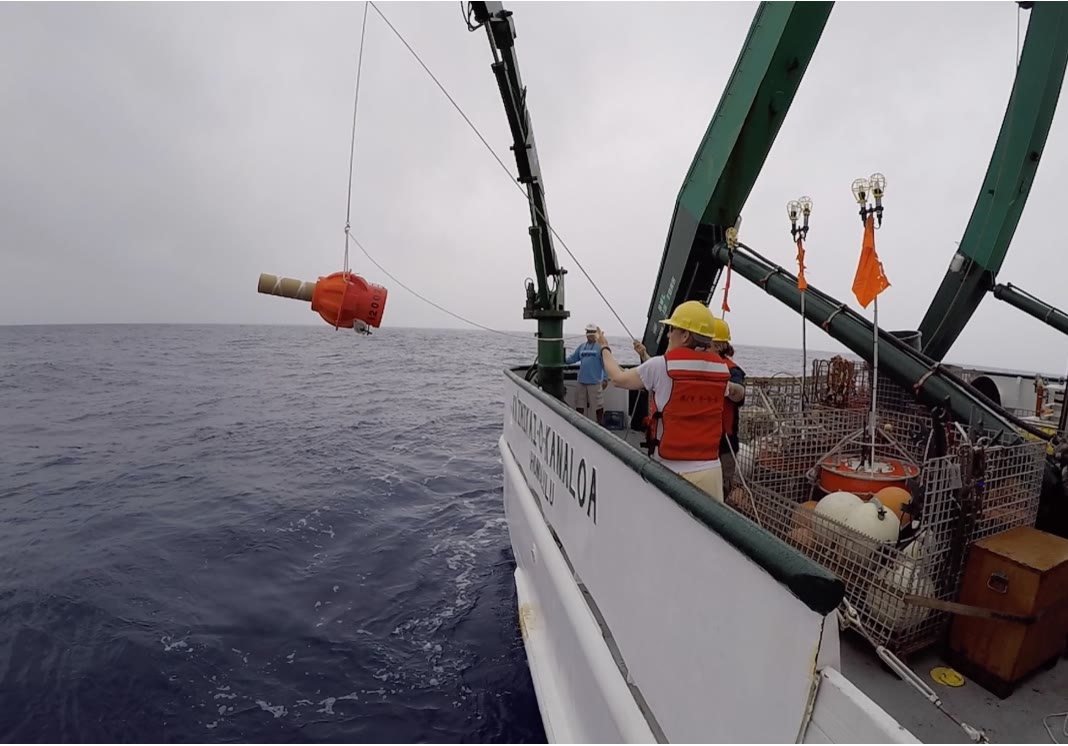
\includegraphics[width=0.6\linewidth]{images/book3/b1-deep-float.jpg}

{\small Un flotador perfilador de océano profundo (el instrumento naranja que cuelga de la grúa) bajado desde un buque de investigación en 2018; una vez liberado, se hunde hasta su profundidad de trabajo y sale a la superficie a intervalos regulares para enviar sus datos. (Fotógrafo no identificado de NOAA, dominio público, vía Wikimedia Commons.)}
\label{fig:b1:ocean-circulation:float}
\end{omfigure}
% ledger: commons:deep-solo, noaa:argo-25

El vuelco transporta calor. El agua que va hacia el norte cálida y vuelve fría ha cedido calor a la atmósfera del norte.

\begin{proposition}[Calor transportado por un vuelco]\label{prop:b1:ocean-circulation:heat}
Si un transporte de volumen $Q$ cruza una \omterm{def:b1:spherical-astronomy:geographic}{latitud} hacia el norte a la \omterm{def:b1:fluid-envelopes-structure:potential-temperature}{temperatura potencial} $\theta_1$ y regresa hacia el sur a $\theta_2$, sin transporte neto de masa, el vuelco lleva hacia el norte el \omterm{def:b1:heat-budget:heat-flow}{flujo de calor}
\[
  H = \rho c_p\,Q\,(\theta_1 - \theta_2),
\]
donde $c_p$ es el calor específico del agua de mar.
\end{proposition}
% ledger: teos10:cp0

\begin{proof}
Cada segundo, la masa $\rho Q$ cruza hacia el norte llevando el contenido de calor $\rho Q
c_p\theta_1$, contado desde un cero arbitrario de temperatura, y la misma masa cruza hacia el sur llevando $\rho Q c_p\theta_2$. El flujo neto hacia el norte es la diferencia; como las dos masas son iguales, el cero arbitrario se cancela, y el resultado es un verdadero transporte de calor.
\end{proof}

Un balance aproximado del Atlántico Norte, de W.~Schmitz, tiene la corriente del Golfo transportando \qty{40}{\sverdrup} de agua a \qty{18}{\celsius} hacia el norte, de los cuales \qty{14}{\sverdrup} regresan hacia el sur como agua profunda a \qty{2}{\celsius}. Con $c_p =
\qty{3992}{J.kg^{-1}.K^{-1}}$ y $\rho = \qty{1027}{kg.m^{-3}}$, este vuelco lleva $1027 \times 3992 \times \num{14e6} \times 16 = \qty{0.92e15}{W}$, unos \qty{0.9}{PW}, hacia el norte de \ang{24} N; estimaciones cuidadosas dan \qty{1.2}{PW}, una cuarta parte del transporte de calor hacia el polo de la atmósfera y el océano combinados. La mayor parte de este calor se entrega al aire sobre el Atlántico Norte septentrional, lo que es una de las razones por las que Noruega, a \ang{60} N, es mucho más cálida que el sur de Groenlandia a la misma \omterm{def:b1:spherical-astronomy:geographic}{latitud}.
% ledger: stewart:heat-conveyor, rapid:home, teos10:cp0 (computed in calc/ch29.py)

La circulación profunda es lenta. Si tarda unos mil años el agua que se hunde en el Atlántico Norte en llegar al Pacífico Norte por la Corriente Circumpolar Antártica, su velocidad media es de unos \qty{1}{mm/s}, cien veces menos que las corrientes profundas variables que registra un correntómetro. Su velocidad se infiere, pues, de trazadores más que medirse: el tritio, liberado a la atmósfera por las pruebas nucleares de los años cincuenta y que decae con una semivida de 12.3 años, entró en el Atlántico Norte profundo donde se forma el agua profunda, y tras 25 años se había extendido poco al sur de \ang{30} N, una velocidad media de menos de \qty{1}{mm/s}. El volumen del océano dividido por la tasa de \omterm{def:b1:ocean-circulation:moc}{formación de agua profunda} da el mismo orden de tiempo (\cref{exo:b1:ocean-circulation:12}).
% ledger: stewart:deep-circulation, nos:conveyor

La Corriente Circumpolar Antártica une las cuencas. Sus corrientes llegan hasta el fondo marino y son lentas, unos \qty{10}{cm/s}, hasta \qty{50}{cm/s} en sus frentes, pero es profunda y ancha: una red de correntómetros fondeados a través del paso de Drake, entre Sudamérica y la Antártida, dio \qty[uncertainty-mode=separate]{125 \pm 11}{\sverdrup} (publicado en 1985), y una red más densa en 2007--2011, que midió también las corrientes cerca del fondo, dio \qty{173.3}{\sverdrup}, un \qty{39}{\percent} más que aquel valor usado durante largo tiempo. Lleva agua profunda de cada océano a los demás y la mezcla en el camino.
% ledger: stewart:acc, donohue:acc

\begin{dated}{2021}
% ledger: ipcc:amoc-observed, ipcc:amoc-projected
La evaluación de 2021 del Grupo Intergubernamental de Expertos sobre el Cambio Climático encuentra, a partir de reconstrucciones, que el vuelco del Atlántico fue relativamente estable en los últimos \num{8000} años (\emph{confianza media}), con un debilitamiento que empieza a finales del siglo XIX (\emph{confianza media}), pero solo tiene \emph{confianza baja} en un descenso global durante el siglo XX. El debilitamiento observado directamente desde mediados de los años 2000 hasta mediados de los 2010 (\emph{confianza alta}) no puede distinguirse de la variabilidad a escala decenal (\emph{confianza alta}). El vuelco es \emph{muy probable} que se debilite durante el siglo XXI en todos los escenarios de emisiones, con solo \emph{confianza baja} en la magnitud del descenso; hay \emph{confianza media} en que no colapsará de forma abrupta antes de 2100.
\end{dated}

\section{Ejercicios}

\begin{exercise}[$\star$]\label{exo:b1:ocean-circulation:1}
Úsese la fórmula de masa con $\rho_a = \qty{1.3}{kg.m^{-3}}$ y el coeficiente de arrastre de Yelland y Taylor. (a)~Calcúlense $C_D$ y la \omterm{def:b1:ocean-circulation:wind-stress}{tensión del viento} para vientos de 4, 7 y
\qty{15}{m/s}. (b)~¿En qué factor crece la tensión de 7 a \qty{15}{m/s}? Compárese con el cociente de los cuadrados de las rapideces y explíquese la diferencia.
% ledger: stewart:wind-stress, stewart:drag-coefficient
\end{exercise}

\begin{exercise}[$\star$]\label{exo:b1:ocean-circulation:2}
Dese la dirección del \omterm{def:b1:ocean-circulation:ekman}{transporte de Ekman} en cada caso. (a)~Un viento que sopla hacia el este a \ang{45} N. (b)~Un alisio del noreste a \ang{15} N. (c)~Un viento que sopla hacia el este a \ang{50} S. (d)~Un viento del sur a lo largo de la costa occidental del sur de África, cerca de \ang{23} S. ¿En cuál de los cuatro casos apunta el transporte mar adentro, y qué se sigue?
\end{exercise}

\begin{exercise}[$\star$]\label{exo:b1:ocean-circulation:3}
A \ang{26.5} N en el Atlántico, los transportes medios de 2004--2024 son: estrecho de Florida \qty{31.7}{\sverdrup}, Ekman \qty{3.5}{\sverdrup}, medio océano superior \qty{-17.9}{\sverdrup}; por capas, de 0 a \qty{800}{m} \qty{16.6}{\sverdrup}, de 800 a \qty{1100}{m} \qty{0.4}{\sverdrup}, de 1100 a \qty{3000}{m} \qty{-12.0}{\sverdrup}, de 3000 a \qty{5000}{m} \qty{-5.9}{\sverdrup} (hacia el norte positivo). (a)~Súmense las tres primeras y compárese con el vuelco publicado, \qty{17.1}{\sverdrup}. (b)~Compárese el flujo hacia el norte por encima de \qty{1100}{m} con el flujo hacia el sur por debajo. (c)~Conviértanse \qty{17.1}{\sverdrup} en kilómetros cúbicos por año, y calcúlese el tiempo que tardaría este flujo en llenar el volumen de todo el océano, \qty{1.3324e9}{km^3}.
% ledger: rapid:transports, charette:ocean-volume
\end{exercise}

\begin{exercise}[$\star$]\label{exo:b1:ocean-circulation:4}
Con las fórmulas de Ekman, calcúlense la profundidad de Ekman y la corriente de superficie bajo un viento de \qty{10}{m/s} a \ang{15}, \ang{45} y \ang{60} de \omterm{def:b1:spherical-astronomy:geographic}{latitud}, y la corriente de superficie como porcentaje del viento. ¿Por qué fallan las fórmulas cerca del ecuador?
% ledger: stewart:ekman-constants
\end{exercise}

\begin{exercise}[$\star\star$]\label{exo:b1:ocean-circulation:5}
A \ang{11} N en el Atlántico, tómese una tensión media del viento de \qty{0.07}{Pa} hacia el oeste sobre un ancho de \qty{5000}{km}, y $\rho = \qty{1027}{kg.m^{-3}}$. (a)~Calcúlese el \omterm{def:b1:ocean-circulation:ekman}{transporte de Ekman} por metro y su dirección. (b)~Calcúlese el transporte de volumen total a través de la sección en \omterm{def:b1:ocean-circulation:ekman}{sverdrups}. (c)~Compárese con los transportes medidos directamente ($12.0 \pm \qty{5.5}{\sverdrup}$) y calculados a partir de vientos de largo plazo ($13.5 \pm \qty{0.3}{\sverdrup}$).
% ledger: stewart:ekman-transport
\end{exercise}

\begin{exercise}[$\star\star$]\label{exo:b1:ocean-circulation:6}
A lo largo del Pacífico ecuatorial, los \omterm{def:b1:atmospheric-circulation:winds}{alisios} ejercen una tensión de \qty{0.05}{Pa} hacia el oeste. (a)~Calcúlese el \omterm{def:b1:ocean-circulation:ekman}{transporte de Ekman} por metro, y su dirección, a \ang{2} N y a \ang{2}~S. (b)~Suponiendo que el agua arrastrada a través de estas dos \omterm{def:b1:spherical-astronomy:geographic}{latitudes} se reemplaza desde abajo entre ellas, calcúlese la velocidad media de \omterm{def:b1:ocean-circulation:upwelling}{afloramiento} en metros por día. (c)~¿Qué ocurre con la fórmula del teorema en el propio ecuador? ¿Qué conclusión sobrevive?
\end{exercise}

\begin{exercise}[$\star\star$]\label{exo:b1:ocean-circulation:7}
Sobre un \omterm{def:b1:ocean-circulation:gyre}{giro subtropical}, tómese una \omterm{def:b1:ocean-circulation:wind-stress}{tensión del viento} de \qty{0.06}{Pa} hacia el oeste a \ang{15} N y \qty{0.12}{Pa} hacia el este a \ang{40} N. (a)~Calcúlense ambos \omterm{def:b1:ocean-circulation:ekman}{transportes de Ekman} y sus direcciones. (b)~Suponiendo que el transporte cambia uniformemente entre las dos \omterm{def:b1:spherical-astronomy:geographic}{latitudes}, calcúlese la velocidad vertical en la base de la \omterm{def:b1:ocean-circulation:ekman}{capa de Ekman}, en metros por año, y dígase si es ascendente o descendente. (c)~Sobre una cuenca de \qty{5000}{km} de ancho, ¿cuántos \omterm{def:b1:ocean-circulation:ekman}{sverdrups} se bombean a través de la base de la capa?
\end{exercise}

\begin{exercise}[$\star\star$]\label{exo:b1:ocean-circulation:8}
Tómese $\rho = \qty{1027}{kg.m^{-3}}$ y $c_p = \qty{3992}{J.kg^{-1}.K^{-1}}$.
(a)~Calcúlese el calor llevado hacia el norte por \qty{17}{\sverdrup} que fluyen hacia el norte a \qty{15}{\celsius} y regresan a \qty{3}{\celsius}. (b)~Compárese con los \qty{1.2}{PW} llevados por el vuelco del Atlántico. (c)~Si la misma agua regresara hacia el sur en la superficie, por el lado oriental de la cuenca, a \qty{12}{\celsius}, ¿qué calor llevaría? ¿Qué dice esto de la importancia de la \omterm{def:b1:ocean-circulation:moc}{formación de agua profunda}?
% ledger: rapid:home, teos10:cp0
\end{exercise}

\begin{exercise}[$\star\star$]\label{exo:b1:ocean-circulation:9}
Tres \omterm{def:b1:fluid-envelopes-structure:ts-diagram}{masas de agua} del Atlántico Sur tienen las \omterm{def:b1:fluid-envelopes-structure:potential-temperature}{temperaturas potenciales} y salinidades siguientes: agua intermedia antártica \qty{3.3}{\celsius}, 34.15; agua profunda del Atlántico Norte \qty{4.0}{\celsius}, 35.00; agua de fondo antártica \qty{0.4}{\celsius}, 34.67. Una muestra a cierta profundidad tiene $\theta = \qty{2.78}{\celsius}$ y $S = 34.731$. Usando \cref{prop:b1:fluid-envelopes-structure:mixing}, calcúlese la fracción de cada \omterm{def:b1:fluid-envelopes-structure:ts-diagram}{masa de agua} en la muestra.
% ledger: stewart:deep-circulation
\end{exercise}

\begin{exercise}[$\star\star\star$]\label{exo:b1:ocean-circulation:10}
Tómese la espiral de \cref{prop:b1:ocean-circulation:spiral}. (a)~Muéstrese que $u$ y $v$
satisfacen $f v + A_z u'' = 0$ y $-f u + A_z v'' = 0$. (Sugerencia: escríbase $u + iv =
V_0\,e^{i\pi/4}\,e^{(1+i)az}$.) (b)~Muéstrese que la tensión $\rho A_z\,\partial\vec
v/\partial z$ en la superficie es igual a la \omterm{def:b1:ocean-circulation:wind-stress}{tensión del viento} $(0, T)$. (c)~Calcúlense los
transportes $\int_{-\infty}^0 \rho u\,\mathrm dz$ y $\int_{-\infty}^0 \rho
v\,\mathrm dz$, y compruébese que concuerdan con
\cref{thm:b1:ocean-circulation:ekman}.
\end{exercise}

\begin{exercise}[$\star\star\star$]\label{exo:b1:ocean-circulation:11}
En el modelo de Stommel, la \omterm{def:b1:ocean-circulation:wbc}{corriente de frontera occidental} tiene un ancho de unos $R/\beta$, donde $R$ es la tasa de fricción en el fondo y $\beta = \mathrm df/\mathrm dy$ la
tasa de aumento hacia el norte del \omterm{def:b1:atmospheric-circulation:coriolis-parameter}{parámetro de Coriolis}. (a)~Muéstrese que $\beta = 2\Omega
\cos\varphi/a_\oplus$ y calcúlese a \ang{30} N ($a_\oplus = \qty{6371}{km}$). (b)~Con $R = \qty{e-6}{s^{-1}}$, calcúlese el ancho. (c)~Un transporte de \qty{30}{\sverdrup} deriva hacia el sur a través del interior de una cuenca de \qty{5000}{km} de ancho en los \qty{1000}{m} superiores, y regresa hacia el norte en la corriente de frontera a lo largo de la misma profundidad. Calcúlense ambas velocidades medias y compárense con la rapidez de la corriente del Golfo, \qty{1.8}{m/s}.
% ledger: stewart:north-atlantic, nos:gulf-stream, earth:Rmean
\end{exercise}

\begin{exercise}[$\star\star\star$]\label{exo:b1:ocean-circulation:12}
El océano contiene \qty{1.3324e9}{km^3} sobre \qty{361.84e6}{km^2}. (a)~Muéstrese que el volumen por debajo de \qty{1000}{m} es al menos de \qty{9.71e8}{km^3}. (b)~El agua profunda del Atlántico Norte se forma a unos \qty{17}{\sverdrup} y el agua de fondo antártica a unos \qty{9}{\sverdrup}. Estímese el tiempo necesario para renovar el agua por debajo de \qty{1000}{m}, y compárese con los mil años de la cinta transportadora. (c)~El tritio tiene una semivida de 12.3 años. ¿Qué fracción de una entrada de tritio queda tras 25 años? ¿Hasta dónde viaja en 25 años el agua que se mueve a \qty{1}{mm/s}?
% ledger: charette:ocean-volume, stewart:deep-circulation, stewart:acc, rapid:transports
\end{exercise}

\section{Problema: una costa de afloramiento}

\begin{problem}[{Problema de fin de semana --- un viento de verano a lo largo de una costa a \ang{38} N}]
\label{pb:b1:ocean-circulation:1}
% values: calc/ch29.py (invented coast; constants from the ledger)
Una costa recta corre de norte a sur a \ang{38} N, con el océano al oeste. En verano, un viento constante de \qty{8}{m/s} sopla desde el norte a lo largo de ella durante semanas. La costa es inventada, pero sus cifras son típicas de los lados orientales de los océanos. Úsense $\Omega = 2\pi/(\qty{23.9345}{h})$, $\rho_a = \qty{1.3}{kg.m^{-3}}$, el coeficiente de arrastre de Yelland y Taylor, $\rho = \qty{1027}{kg.m^{-3}}$ para el agua de mar y $c_p = \qty{3992}{J.kg^{-1}.K^{-1}}$.

\medskip
\noindent\textbf{Parte I --- El viento y su tensión.}
\begin{enumerate}
  \item ¿Hacia qué dirección sopla el viento? ¿Es a lo largo de la costa o a través de ella?
  \item Calcúlese el coeficiente de arrastre.
  \item Calcúlese la \omterm{def:b1:ocean-circulation:wind-stress}{tensión del viento}.
  \item Lo mismo para un viento de \qty{12}{m/s}. ¿En qué factor crece la tensión, y por qué es más que el cociente de los cuadrados de las rapideces?
  \item Calcúlese el \omterm{def:b1:atmospheric-circulation:coriolis-parameter}{parámetro de Coriolis} a \ang{38} N.
  \item Calcúlese $2\pi/f$ en horas. ¿Por qué el viento debe soplar un día o más antes de que se aplique el equilibrio de Ekman?
\end{enumerate}

\medskip
\noindent\textbf{Parte II --- La capa de Ekman.}
\begin{enumerate}[resume]
  \item ¿En qué dirección está el \omterm{def:b1:ocean-circulation:ekman}{transporte de Ekman}? ¿Hacia la tierra o hacia el mar abierto?
  \item Calcúlese el transporte de masa de Ekman por metro de costa.
  \item Conviértase en un transporte de volumen por metro.
  \item Calcúlese la profundidad de Ekman con la fórmula de Ekman.
  \item Calcúlese la velocidad media mar adentro en la capa, en \unit{cm/s}.
  \item Calcúlese la corriente de superficie con la fórmula de Ekman, y su dirección. ¿Qué sugieren en cambio las medidas de las boyas sobre su rapidez?
\end{enumerate}

\medskip
\noindent\textbf{Parte III --- Afloramiento en la costa.}
\begin{enumerate}[resume]
  \item Explíquese, con un esquema de una sección vertical, de dónde procede el agua arrastrada mar adentro.
  \item Calcúlese el volumen afluido por día a lo largo de cada kilómetro de costa.
  \item Supóngase que el agua sube a través de una banda de \qty{20}{km} de ancho a lo largo de la costa. Calcúlese la velocidad media ascendente, en \unit{m/s} y en metros por día.
  \item ¿Cuánto tarda el agua en subir desde la base de la \omterm{def:b1:ocean-circulation:ekman}{capa de Ekman} hasta la superficie a esta velocidad?
  \item El agua afluida llega a la superficie a \qty{12}{\celsius}, mientras que el mar abierto mar adentro está a \qty{18}{\celsius}. La brisa marina lleva aire cálido y húmedo desde mar adentro sobre esta agua. ¿Qué le ocurre al aire cerca de la superficie, y qué tiempo sigue en la costa?
  \item ¿Por qué son ricas en peces estas costas?
  \item En otoño el viento cambia y sopla desde el sur durante una semana. ¿Qué ocurre con el transporte y con el agua de la costa?
\end{enumerate}

\medskip
\noindent\textbf{Parte IV --- Otras costas y el transporte total.}
\begin{enumerate}[resume]
  \item Con la misma tensión, calcúlese el \omterm{def:b1:ocean-circulation:ekman}{transporte de Ekman} por metro a \ang{20} N y compárese con el de \ang{38} N.
  \item En la costa occidental del sur de África, cerca de \ang{23} S, ¿qué dirección del viento impulsa el \omterm{def:b1:ocean-circulation:upwelling}{afloramiento}? Compárese con la costa del problema.
  \item Con un viento de \qty{5}{m/s} en lugar de \qty{8}{m/s} a \ang{38} N, calcúlense la tensión y el \omterm{def:b1:ocean-circulation:ekman}{transporte de Ekman} por metro, y su cociente con los de la pregunta~8.
  \item El agua afluida se calienta \qty{6}{\celsius} al alejarse mar adentro. Calcúlese el calor que toma por segundo y por metro de costa, y después a lo largo de \qty{1000}{km}.
  \item ¿Qué longitud de una costa así afloraría tanta agua como la que lleva la corriente del Golfo por el estrecho de Florida, \qty{31.7}{\sverdrup}?
  \item ¿Qué volumen de agua, en \omterm{def:b1:ocean-circulation:ekman}{sverdrups}, aflora a lo largo de \qty{1000}{km} de esta costa?
\end{enumerate}
\end{problem}
